\documentclass[11pt,letterpaper]{article}

\usepackage[spanish]{babel}
\usepackage[utf8]{inputenc}
\usepackage[T1]{fontenc}
\usepackage{geometry}
\usepackage{graphicx}
\usepackage{booktabs}
\usepackage{float}
\usepackage{hyperref}
\usepackage{array}
\usepackage{xcolor}

\geometry{margin=2.4cm}
\hypersetup{
    colorlinks=true,
    linkcolor=blue,
    urlcolor=blue
}

\title{Tarea 2: Procesamiento Asíncrono y Fallback con Apache Kafka}
\author{Sebastián León}
\date{Sistemas Distribuidos 2026-1}

\begin{document}

\maketitle

\section{Introducción}

En la Tarea 1 se implementó una plataforma distribuida para consultas geoespaciales sobre el dataset Google Open Buildings, utilizando Redis como sistema de caché. En esta segunda entrega se evoluciona la arquitectura para incorporar Apache Kafka como cola de mensajes entre el generador de tráfico y el procesamiento de consultas. El objetivo es desacoplar la llegada de solicitudes respecto del Generador de Respuestas, tolerar fallas temporales mediante reintentos, registrar consultas no recuperables en una Dead Letter Queue (DLQ) y evaluar el impacto del procesamiento paralelo con múltiples consumidores.

El sistema mantiene las consultas Q1--Q5 y las distribuciones Zipf/uniforme de la Tarea 1. La diferencia principal es que, en la arquitectura Kafka, el Generador de Tráfico ya no invoca directamente el procesamiento, sino que publica mensajes en un tópico principal. Los consumidores Kafka procesan esos mensajes, consultan Redis, ejecutan el Generador de Respuestas ante cache miss y reenvían mensajes fallidos a un tópico de reintentos.

\section{Arquitectura del sistema}

La arquitectura implementada mantiene los componentes originales y agrega una capa de mensajería Kafka. Los componentes principales son:

\begin{itemize}
    \item \textbf{Generador de Tráfico}: genera consultas Q1--Q5 con distribución Zipf o uniforme.
    \item \textbf{Kafka Producer}: publica las consultas en el tópico principal \texttt{geo-queries}.
    \item \textbf{Kafka Consumers}: consumen desde \texttt{geo-queries} y \texttt{geo-queries-retry}, todos dentro del grupo \texttt{geo-workers}.
    \item \textbf{Sistema Caché}: Redis almacena respuestas ya calculadas.
    \item \textbf{Generador de Respuestas}: reutiliza las funciones Q1--Q5 para resolver cache misses.
    \item \textbf{Tópico de Reintentos}: \texttt{geo-queries-retry} recibe consultas con fallas temporales.
    \item \textbf{Dead Letter Queue}: \texttt{geo-queries-dlq} recibe consultas que superan el máximo de reintentos.
    \item \textbf{Monitor de Backlog}: registra periódicamente mensajes pendientes en Kafka.
    \item \textbf{Sistema de Métricas}: almacena métricas agregadas en Redis para permitir múltiples consumidores.
\end{itemize}

\subsection{Flujo de procesamiento}

Cada consulta publicada por el productor incluye un identificador único, el número de intentos realizados, el timestamp de creación y los parámetros de la consulta. El consumidor primero consulta Redis. Si existe cache hit, registra éxito inmediatamente. Si ocurre cache miss, invoca el Generador de Respuestas. Las fallas temporales se simulan mediante una probabilidad de error o una ventana de indisponibilidad. En ese caso, el mensaje se reenvía al tópico de reintentos. Si el número de intentos supera el máximo configurado, el mensaje se envía a la DLQ.

\section{Decisiones de diseño}

\subsection{Estrategia de reintentos}

Se utiliza un único tópico de reintentos, \texttt{geo-queries-retry}, y un máximo de 3 reintentos por consulta. Cada mensaje mantiene el campo \texttt{attempts}, por lo que los consumidores pueden decidir si reintentar o enviar a DLQ sin depender de estado local. Esta decisión simplifica el análisis experimental y evita que un fallo temporal cause pérdida inmediata de consultas.

La condición de DLQ es: si una consulta falla y \texttt{attempts} supera el máximo configurado, se publica en \texttt{geo-queries-dlq}. En los experimentos ejecutados no se observaron mensajes en DLQ, lo que indica que las fallas simuladas fueron transitorias y recuperables dentro del límite de intentos.

\subsection{Configuración de caché}

Redis se configura con 200 MB y política \texttt{allkeys-lru}. Se eligió LRU porque el tráfico Zipf genera repetición de zonas y tipos de consulta, por lo que mantener en caché las claves usadas recientemente es una política razonable. El TTL se mantiene diferenciado por tipo de consulta:

\begin{center}
\begin{tabular}{cc}
\toprule
Consulta & TTL \\
\midrule
Q1 & 60 s \\
Q2 & 60 s \\
Q3 & 120 s \\
Q4 & 120 s \\
Q5 & 90 s \\
\bottomrule
\end{tabular}
\end{center}

\subsection{Procesamiento paralelo}

Los consumidores pertenecen al mismo grupo \texttt{geo-workers}. Kafka distribuye particiones entre los consumidores disponibles, permitiendo balanceo automático. Los tópicos se crean con 6 particiones, lo que permite que escenarios con 1, 2 y 4 consumidores tengan particiones suficientes para paralelizar el procesamiento.

\section{Metodología experimental}

Se evaluaron dos familias de experimentos. Primero, se usa la arquitectura síncrona de la Tarea 1 como línea base. Segundo, se ejecutan escenarios Kafka con 1000 consultas por escenario, distribución Zipf, seed fija y distintos patrones de carga/falla.

Los escenarios Kafka fueron:

\begin{itemize}
    \item Kafka con 1 consumer.
    \item Kafka con 2 consumers.
    \item Kafka con 4 consumers.
    \item Falla temporal del Generador de Respuestas.
    \item Reintentos por fallas aleatorias.
    \item Spike de tráfico.
\end{itemize}

Las métricas registradas fueron throughput, latencia p50/p95, retry rate, recovery rate, DLQ rate, backlog máximo y cantidad de consultas recuperadas.

\section{Resultados}

\subsection{Arquitectura síncrona base}

Como línea base se consideran los experimentos de la Tarea 1 con Redis LRU y 200 MB. Los resultados fueron:

\begin{table}[H]
\centering
\begin{tabular}{lrrrrr}
\toprule
Distribución & Consultas & Throughput & p50 & p95 & Hit rate \\
\midrule
Zipf & 10000 & 1818.42 req/s & 0.17 ms & 0.75 ms & 75.8\% \\
Uniforme & 10000 & 887.18 req/s & 0.64 ms & 1.18 ms & 67.5\% \\
\bottomrule
\end{tabular}
\caption{Resultados base de arquitectura síncrona con Redis LRU 200 MB.}
\end{table}

La arquitectura síncrona tiene latencias muy bajas porque el flujo ocurre dentro del mismo proceso de simulación y no incluye espera en cola. Sin embargo, ante fallas del Generador de Respuestas, las consultas no quedan protegidas por una cola persistente.

\subsection{Resultados con Kafka}

\begin{table}[H]
\centering
\small
\begin{tabular}{lrrrrrrr}
\toprule
Escenario & Cons. & Exitosas & Throughput & p50 & p95 & Retry & DLQ \\
\midrule
Kafka 1 consumer & 1 & 1000 & 20.22 & 35831.80 & 41050.97 & 0.0\% & 0.0\% \\
Kafka 2 consumers & 2 & 1000 & 22.13 & 33434.30 & 36700.41 & 0.0\% & 0.0\% \\
Kafka 4 consumers & 4 & 1000 & 14.84 & 56260.90 & 59062.93 & 0.0\% & 0.0\% \\
Falla temporal & 2 & 1000 & 21.46 & 35749.36 & 39535.43 & 1.6\% & 0.0\% \\
Reintentos & 2 & 1000 & 16.16 & 41655.00 & 52450.50 & 13.9\% & 0.0\% \\
Spike tráfico & 2 & 1000 & 23.02 & 32567.82 & 34956.24 & 0.0\% & 0.0\% \\
\bottomrule
\end{tabular}
\caption{Resultados experimentales con arquitectura Kafka. Latencias en milisegundos.}
\end{table}

\begin{figure}[H]
\centering
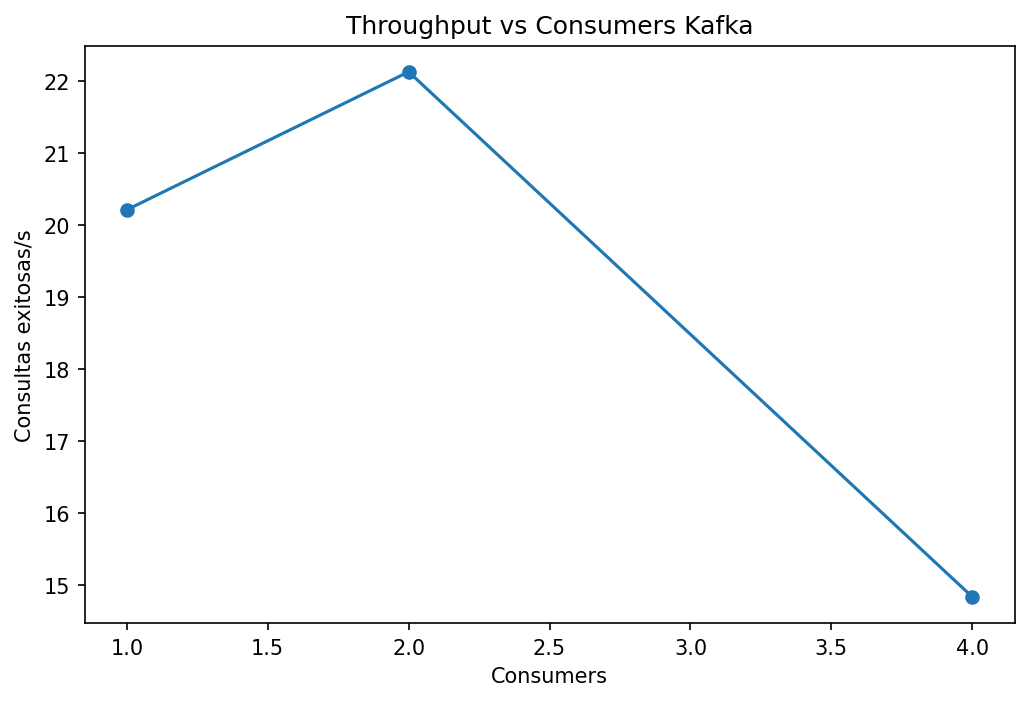
\includegraphics[width=0.8\textwidth]{experiment_results_kafka/01_throughput_consumers.png}
\caption{Throughput al variar la cantidad de consumidores Kafka.}
\end{figure}

\begin{figure}[H]
\centering
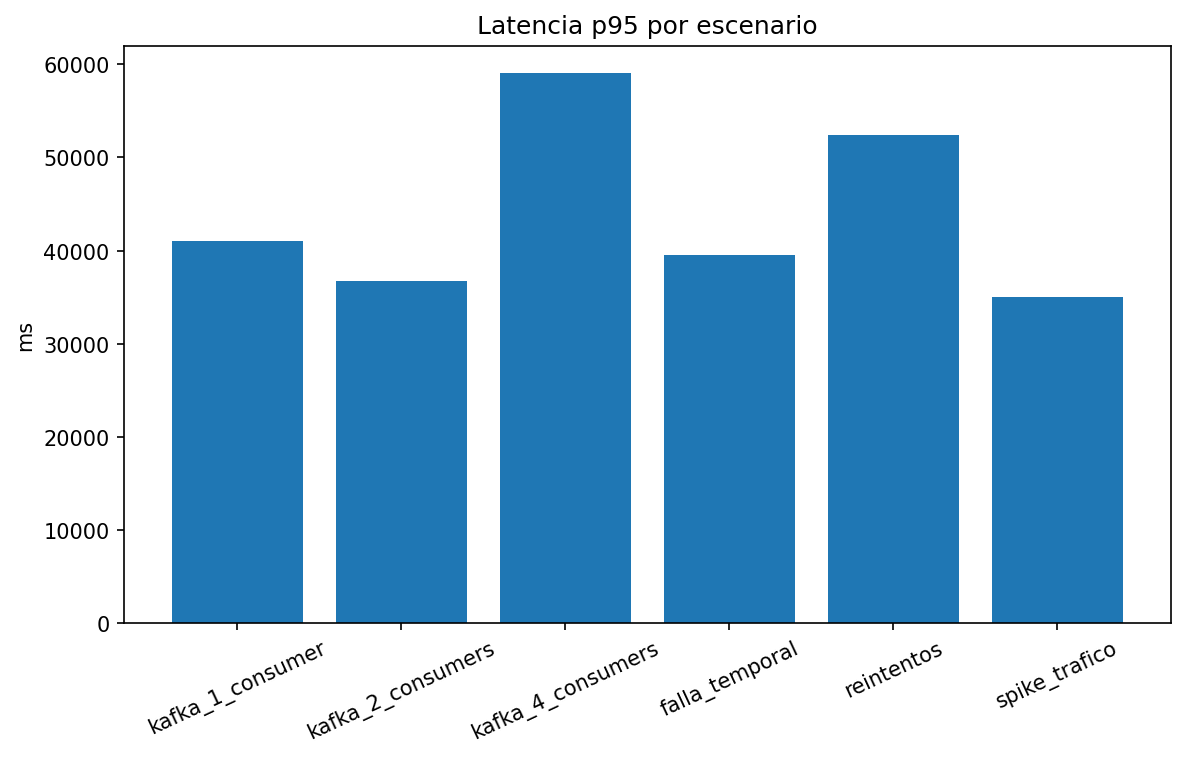
\includegraphics[width=0.8\textwidth]{experiment_results_kafka/02_latencia_p95_escenarios.png}
\caption{Latencia p95 por escenario.}
\end{figure}

\begin{figure}[H]
\centering
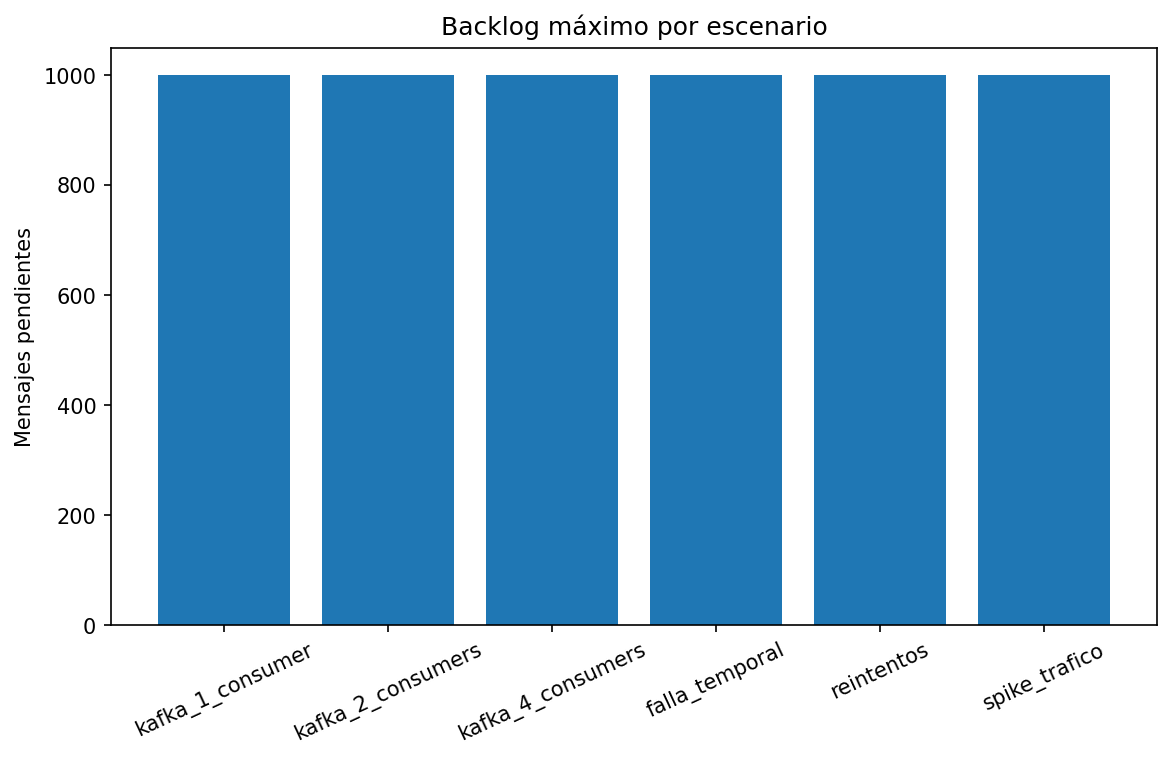
\includegraphics[width=0.8\textwidth]{experiment_results_kafka/03_backlog_maximo.png}
\caption{Backlog máximo observado por escenario.}
\end{figure}

\begin{figure}[H]
\centering
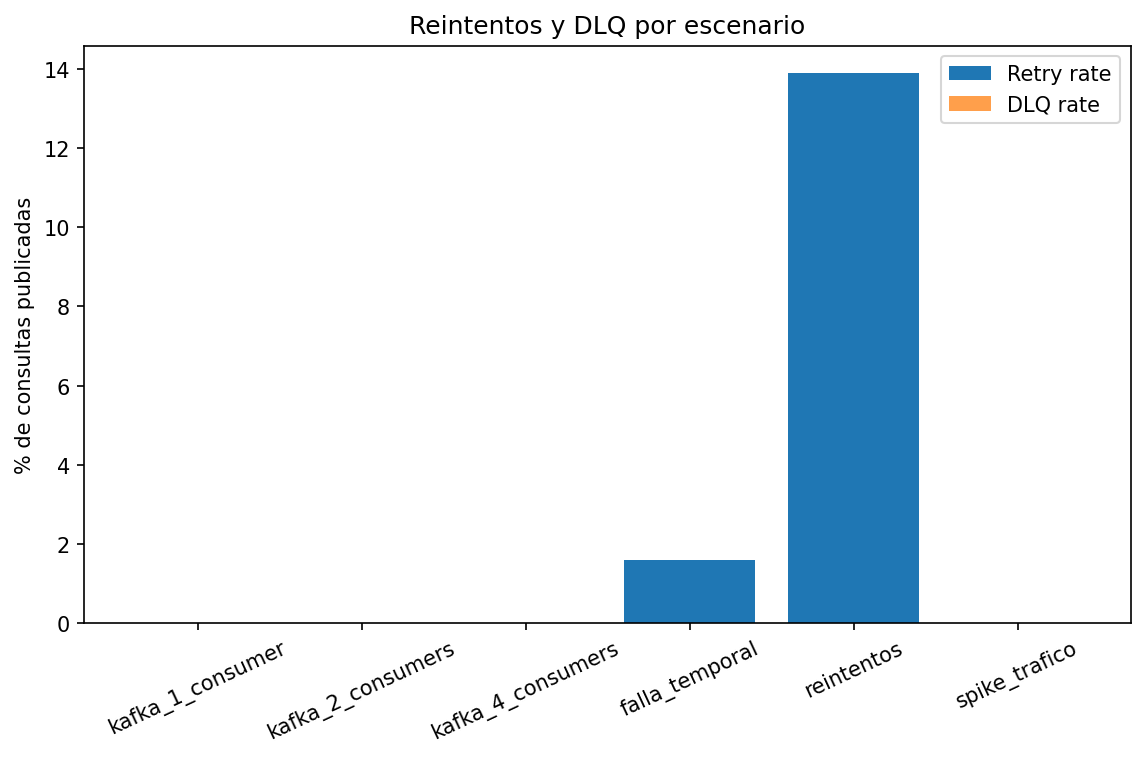
\includegraphics[width=0.8\textwidth]{experiment_results_kafka/04_retry_dlq_rates.png}
\caption{Retry rate y DLQ rate por escenario.}
\end{figure}

\section{Análisis}

\subsection{Comparación entre arquitectura síncrona y Kafka}

La arquitectura síncrona presenta mayor throughput y menor latencia en condiciones normales. Esto ocurre porque evita la sobrecarga de serialización, publicación, consumo y confirmación de offsets en Kafka. Además, las mediciones síncronas no incluyen espera en cola. En cambio, la arquitectura Kafka mide latencia end-to-end desde la creación del mensaje hasta su resolución, por lo que incluye tiempo en tópico, espera por consumidores y procesamiento.

La ventaja de Kafka no está en reducir la latencia mínima, sino en mejorar la resiliencia. Si el Generador de Respuestas falla temporalmente, las consultas no se pierden inmediatamente; quedan en Kafka o pasan al tópico de reintentos. Esto permite recuperar consultas cuando el servicio vuelve a estar disponible, a cambio de una mayor latencia total.

\subsection{Impacto de consumidores paralelos}

Al pasar de 1 a 2 consumidores, el throughput aumenta de 20.22 a 22.13 consultas/s y la latencia p95 baja de 41050.97 ms a 36700.41 ms. Esto muestra beneficio por paralelismo. Sin embargo, con 4 consumidores el throughput baja a 14.84 consultas/s y la latencia p95 sube a 59062.93 ms. Esto sugiere que el sistema no escala linealmente. La causa probable es la sobrecarga de cargar el dataset en memoria en cada consumidor, competencia por CPU/memoria y acceso compartido a Redis. Por lo tanto, más consumidores no siempre implican mejor desempeño si el recurso limitante deja de ser Kafka.

\subsection{Reintentos, recuperación y DLQ}

En el escenario de falla temporal se registraron 16 reintentos y 16 recuperaciones, con recovery rate de 100\%. Esto indica que la cola de reintentos logró absorber fallas transitorias sin pérdida de consultas. En el escenario de fallas aleatorias hubo 139 reintentos, 123 consultas recuperadas y 0 mensajes en DLQ. El retry rate subió a 13.9\% y la latencia p95 aumentó a 52450.50 ms. Esto muestra el trade-off principal: los reintentos reducen pérdida de consultas, pero aumentan la latencia total.

La DLQ no recibió mensajes durante estos experimentos. Esto es positivo para los escenarios probados, pero también implica que para demostrar explícitamente la DLQ en el video conviene ejecutar una corrida con \texttt{--failure-rate 1.0} y \texttt{--max-attempts 1}, de modo que algunas consultas superen el límite de reintentos.

\subsection{Backlog, fallas y spike de tráfico}

El backlog máximo observado fue 1000 mensajes en los escenarios Kafka. Esto ocurre porque el productor puede publicar consultas más rápido que la velocidad inicial de consumo, especialmente considerando que cada consumidor carga el dataset completo antes de procesar. Luego, los consumidores vacían progresivamente la cola. Este comportamiento es esperable en arquitecturas basadas en colas: Kafka desacopla llegada y procesamiento, permitiendo absorber spikes, pero la latencia crece si el ritmo de llegada supera temporalmente la capacidad de consumo.

En el escenario de spike de tráfico se obtuvo el mayor throughput observado con 2 consumidores, 23.02 consultas/s, y latencia p95 de 34956.24 ms. El sistema no perdió consultas, lo que evidencia que Kafka actuó como buffer. En un sistema síncrono, un spike similar presionaría directamente al Generador de Respuestas y aumentaría la probabilidad de timeouts o pérdida de solicitudes.

\section{Ventajas y desventajas de la arquitectura con colas}

\subsection{Ventajas}

\begin{itemize}
    \item Desacopla generación y procesamiento de consultas.
    \item Permite recuperación automática ante fallas temporales.
    \item Soporta múltiples consumidores en paralelo.
    \item Permite observar backlog y comportamiento bajo sobrecarga.
    \item La DLQ separa mensajes problemáticos sin bloquear el flujo principal.
\end{itemize}

\subsection{Desventajas}

\begin{itemize}
    \item Aumenta la complejidad operacional.
    \item Aumenta latencia end-to-end por espera en cola.
    \item Requiere monitorear tópicos, offsets y consumidores.
    \item El escalamiento horizontal puede quedar limitado por CPU, memoria, Redis o carga del dataset.
\end{itemize}

\section{Reproducibilidad}

El sistema completo se despliega con Docker Compose:

\begin{verbatim}
docker compose --profile kafka up -d redis kafka
docker compose --profile kafka run --rm kafka-consumer
docker compose --profile kafka run --rm kafka-producer python kafka_producer.py
python run_kafka_experiments.py
\end{verbatim}

Los resultados experimentales se guardan en \texttt{experiment\_results\_kafka/}. El dataset no se incluye en el repositorio por tamaño; debe ubicarse en \texttt{app/data/967\_buildings.csv.gz}.

\section{Conclusión}

La incorporación de Kafka transforma el sistema desde una arquitectura síncrona de baja latencia hacia una arquitectura asíncrona más tolerante a fallos. Los experimentos muestran que Kafka introduce mayor latencia y menor throughput en condiciones normales, pero permite recuperar consultas ante fallas temporales y absorber spikes mediante backlog. El sistema implementa tópicos de reintento, DLQ, consumidores paralelos y métricas completas, cumpliendo los objetivos principales de la Tarea 2.

\end{document}
